\chapter{Resultados Experimentales y Discusión}
\label{Resultados Experimentales y Discusión}
\section{Comportamiento de Conversor}
Esto es solo texto para ver el espacio de texto disponible para escribor. Aca se explicara como la resistencia de 100 Ohms ayuda a que el sobrepulso no romba el gate  del mosfet p
\begin{figure}[h!]
    \centering
    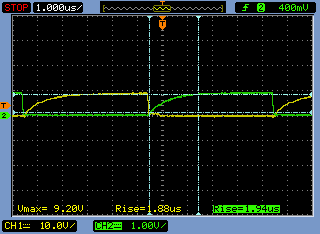
\includegraphics[width=1\linewidth]{imagenes/testosc0.png}
    \caption{Voltaje en Gate de Mosfets}
    \label{fig:tension_gate_mosfets}
\end{figure}
or estres, bajar el ruido, y baja la corriente exigida al driver. Tambien se explica como la resistencia de 10 Ohm quemo el driver. Como se ve en el impreso, imagenes ocupan bastante espacio si se deja al ratio de el ancho de escritura.
\subsection{Respuesta transitoria}
\begin{figure}[H]
    \centering
    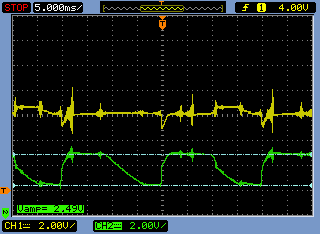
\includegraphics[width=1\linewidth,frame]{imagenes/testosc4.png}
    \caption{Respuesta transitoria de conversor en Laboratorio}
    \label{fig:resp_tran_lab}
\end{figure}
\section{Eficiencia}
La eficiencia del conversor Buck esta ligada al duty-cycle que le controla, por lo que un barrido de este conectado en el panel solar de campo se obtiene la figura \ref{fig:efficiency_solar_panel}.
\begin{figure}[H]
    \centering
    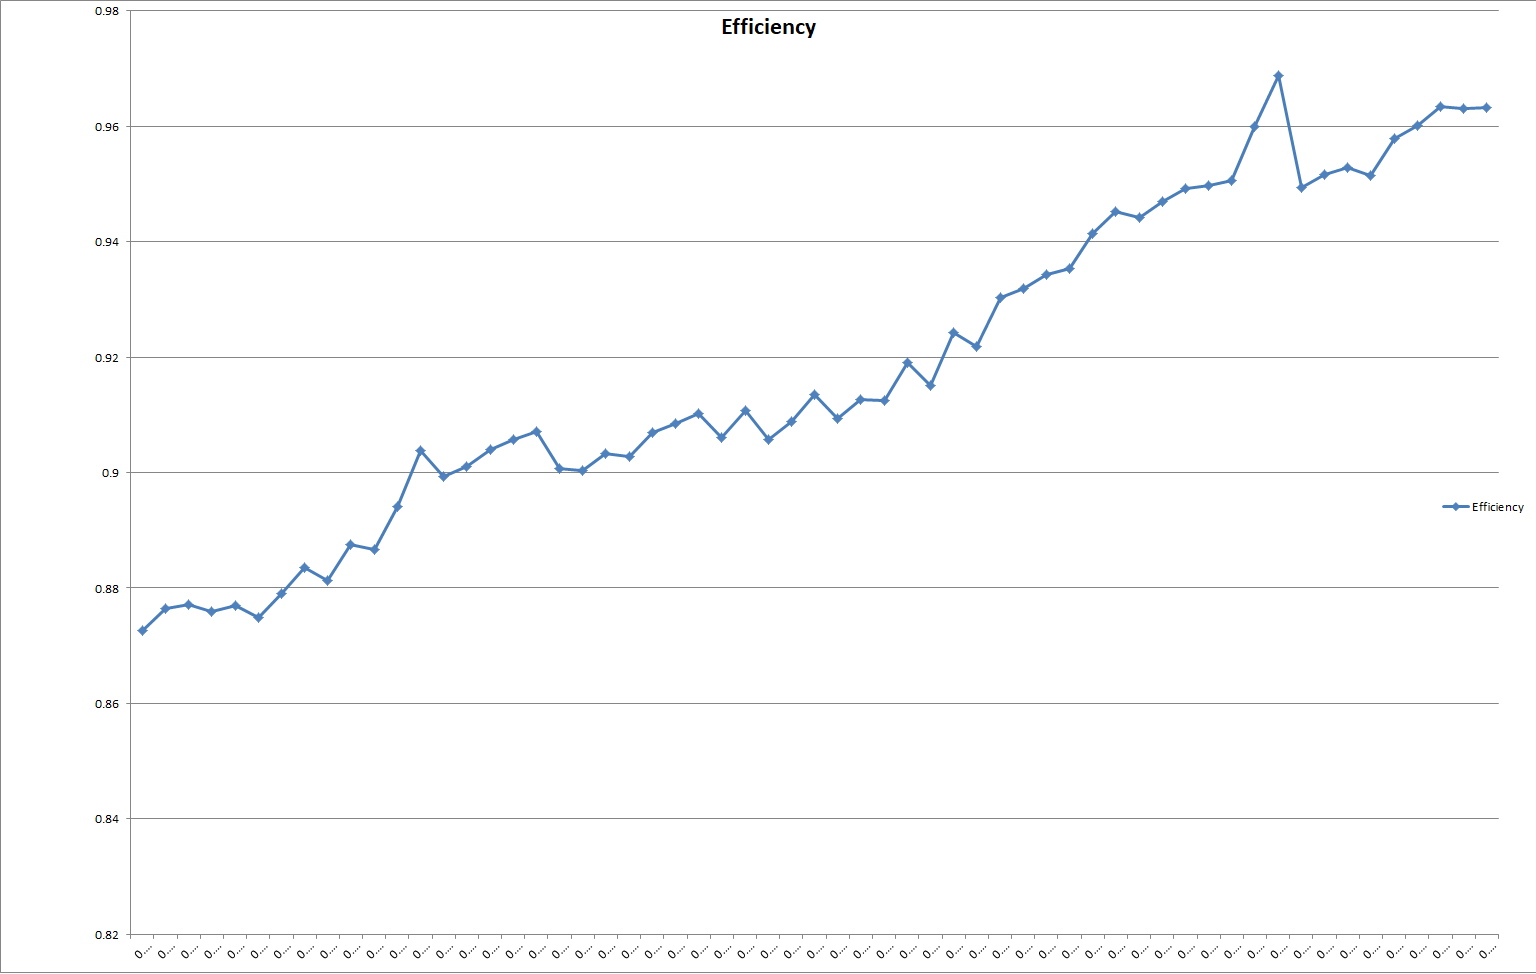
\includegraphics[width=1\linewidth]{imagenes/efficiency.png}
    \caption{Eficiencia de conversor Buck en campo}
    \label{fig:efficiency_solar_panel}
\end{figure}
\section{Condición de sombreado parcial}
\section{Respuesta de los métodos MPPT}
Con un barrido de duty-cycle en sistema real a través de la placa esp32 ,y calculo en tabla de excel posterior, se realiza las conclusiones, desarrollo, y modificaciones a los métodos en base a la curva de la Figura \ref{fig:curva_panel_esp32}.
\begin{figure}[H]
    \centering
    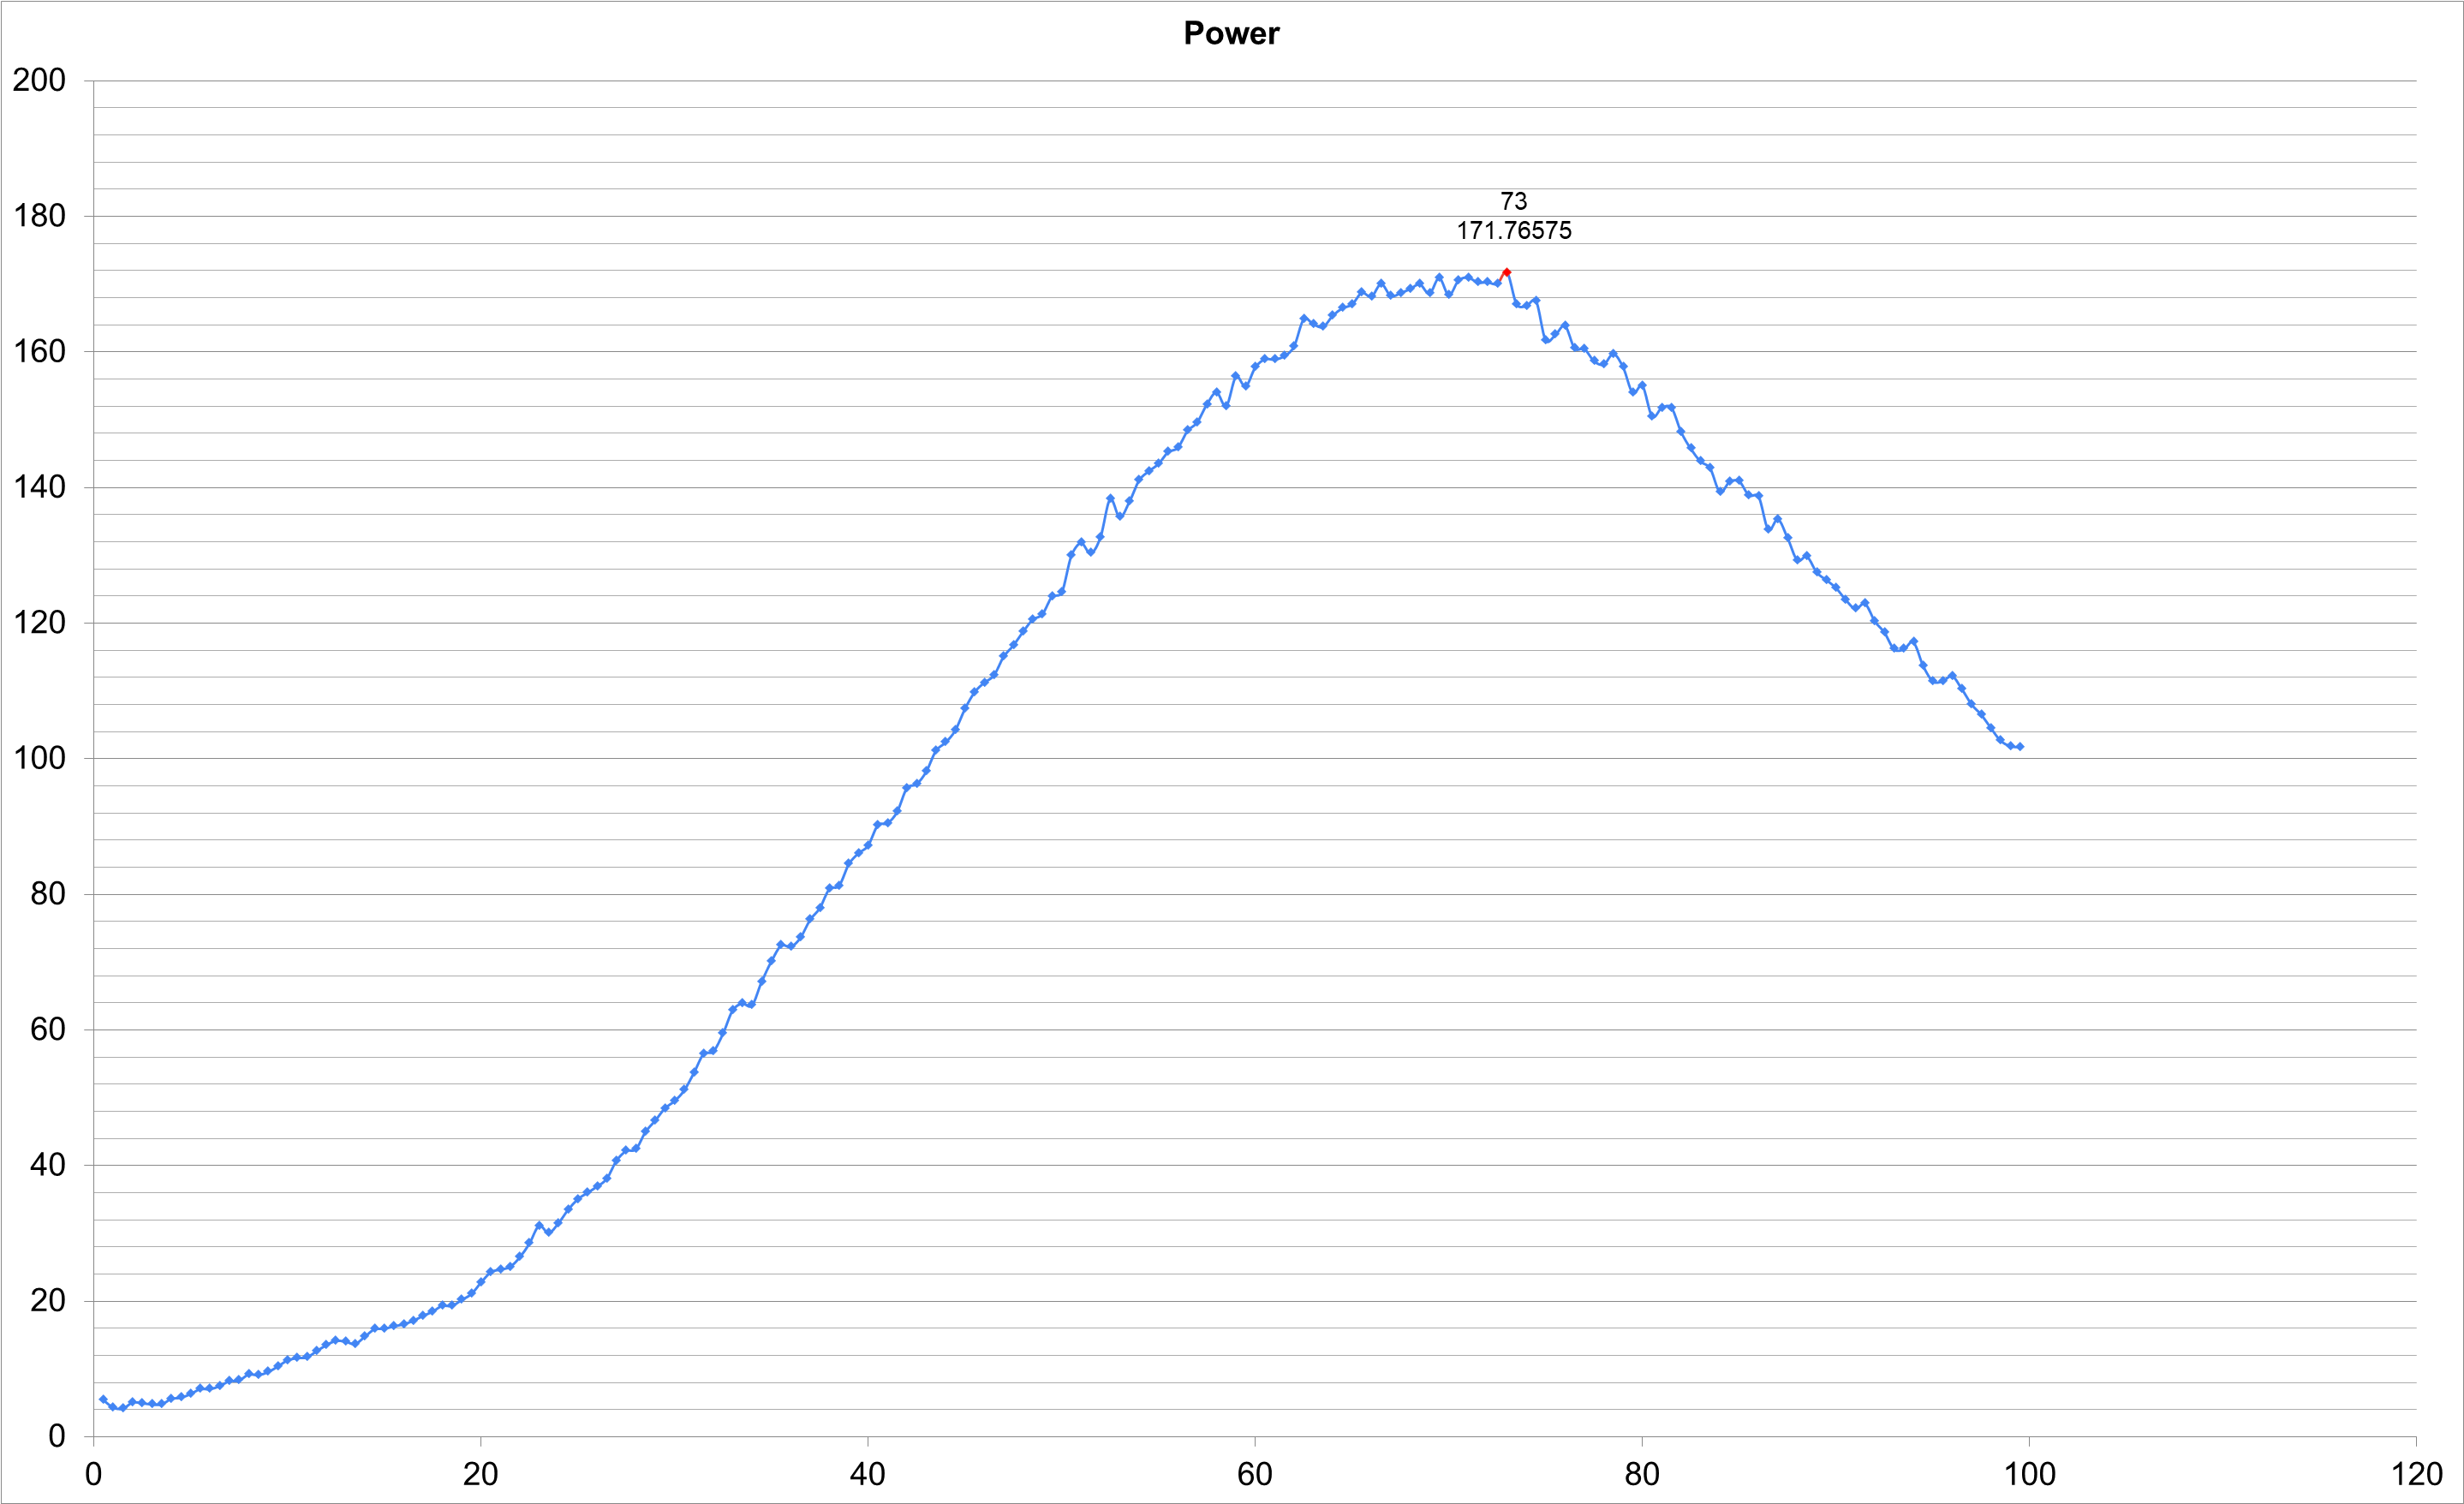
\includegraphics[width=1\linewidth]{imagenes/curva_panel_solar_por_esp32.png}
    \caption{Curva característica de panel solar a través de ESP32}
    \label{fig:curva_panel_esp32}
\end{figure}
(Texto debajo de imagen para corroborar espacio. Posible problema a futuro en formato, el cual no se esta pensando por ahora hasta terminar los escritos)
